%%%%%%%%%%%%%%%%%%%%%%%%%%%%%%%%%%%%%%%%%%%%%%%%%%%%%%%%%%%%%%%%%%%%%
%%                                                                 %%
%% Please do not use \input{...} to include other tex files.       %%
%% Submit your LaTeX manuscript as one .tex document.              %%
%%                                                                 %%
%%%%%%%%%%%%%%%%%%%%%%%%%%%%%%%%%%%%%%%%%%%%%%%%%%%%%%%%%%%%%%%%%%%%%

\documentclass[pdflatex,mathphys]{jnl}

\usepackage{caption}
\usepackage{graphicx}
\usepackage{subcaption}
\usepackage{overpic}
\captionsetup{justification=justified, font=small}

\usepackage{paralist}

\usepackage{siunitx}

\raggedbottom

% ============================================================================
% FIGURE STRUCTURE (driven by the BoG 2026 talk deck + transcript):
%   Fig 1  Genome-wide subtelomeric homology + PHR extent        (deck slides 3,4)
%   Fig 2  Pangenome similarity structure + communities          (deck slides 6,10,12)
%   Fig 3  Architecture of representative communities (browser)  (deck slides 14,15,16)
%   Fig 4  Sequence similarity predicts 3D proximity             (deck slides 20,21,22)
%          a HG002 Pore-C all-points scatter; b Pore-C community matrix; c mouse bouquet
%   Fig 5  Pedigree-resolved subtelomeric exchange (untangle)    (deck slides 24,26)
% Extended Data: ED1 = 3-panel replicate of Fig 4a across genomes/assays (CHM13
% Hi-C, HG002 Hi-C, HG002 CiFi), all 50 kbp all-points. The mouse
% meiotic-bouquet result is Fig 4c; other reviewer-era analyses remain as text.
% Figure-generation workflows are provided in the public analysis-code repository.
% ============================================================================

\begin{document}

\title[Concerted evolution and unorthodox recombination of human subtelomeres]{Concerted evolution and unorthodox recombination of human subtelomeres}

\author*[1]{\fnm{Andrea} \sur{Guarracino}}\email{aguarracino@tgen.org}
\author[2]{\fnm{Angela} \sur{Gyamfi}}
\author*[3]{\fnm{Erik} \sur{Garrison}}\email{egarris5@uthsc.edu}

\affil[1]{Bioinnovation and Genome Sciences, The Translational Genomics Research Institute (TGen), Phoenix, AZ 85004, USA}
\affil[2]{St. Jude Children's Research Hospital, Memphis, TN 38105, USA}
\affil[3]{Department of Genetics, Genomics and Informatics, University of Tennessee Health Science Center, 71 S Manassas St, Memphis, 38163, Tennessee, USA}

\abstract{
Human chromosome ends are often treated as chromosome-specific, yet much of their subtelomeric sequence is shared with the ends of other, non-homologous chromosomes. Here we measure this sharing across 465 near-complete assemblies (464 HPRC v2 haplotypes from 232 individuals, together with CHM13) using an implicit pangenome graph that samples approximately 12\% of haplotype-pair comparisons and queries transitive relationships without chromosomal or positional priors. We find extended interchromosomal homology on 41 of 48 chromosome arms, spanning tens to hundreds of kilobases and totaling 3.51 Mb outside acrocentric short arms and pseudoautosomal regions. These pseudo-homolog regions form 15 arm-level sequence-similarity communities, with known systems and an enriched q-arm neighborhood appearing as localized high-similarity peaks on a broader subtelomeric similarity continuum. Human and mouse contact maps support increased three-dimensional proximity among sequence-similar subtelomeres during interphase and meiotic prophase I. A telomere-to-telomere human pedigree provides evidence consistent with recent exchange preferentially within these sequence communities. Together, these data identify pseudo-homologous subtelomeres as a near-ubiquitous feature of human chromosome ends and support a model in which nuclear architecture and recombination opportunity contribute to their concerted evolution.
}

\keywords{pangenome, subtelomere, pseudo-homolog region, concerted evolution, recombination, Hi-C, meiotic bouquet, HPRC v2}

\maketitle

Human subtelomeres are among the most rearrangement-prone and fast-evolving
regions of the human genome. Cytogenetic and clone-based studies established that each chromosome end is a
mosaic of duplicated segments also found at the ends of several other,
non-homologous chromosomes, arranged in two domains: proximal,
chromosome-specific sequence and a distal zone of repeats shared across many
ends \cite{MeffordTrask2002,Flint1997,Linardopoulou2005}.
Duplication of these blocks gave rise to subtelomere-specific gene families
(olfactory receptors, tubulins and the D4Z4/DUX4 macrosatellite) and left their
copy number and sequence variable within and between human populations
\cite{MeffordTrask2002}.
These ends also exchange sequence ectopically, by translocation and gene
conversion \cite{Brown1990,Wilkie1991,Trask1991}, and that exchange has
continued into recent human evolution, with a large fraction of subtelomeric
sequence having arisen from duplications specific to the human lineage
\cite{Linardopoulou2005}.

This ectopic exchange has well-known consequences at particular chromosome ends.
The pseudoautosomal regions PAR1 and PAR2 carry the obligate sex-chromosome
crossover \cite{Rouyer1986,sexchrompars_bellott2024}; the ribosomal-DNA-bearing
acrocentric short arms recombine in the nucleolus and underlie recurrent
Robertsonian translocations
\cite{acrocentric_Altemose2022,acrocentric_Guarracino2025ape}; the D4Z4
macrosatellite of 4q35 and 10q26 causes facioscapulohumeral dystrophy and is
reactivated in diverse cancers
\cite{dux4_d4z4_fshd_lemmers2010worldwide,dux4_cancer_Chew2019}; and unbalanced
subtelomeric rearrangements are a recurrent cause of intellectual disability
\cite{MeffordTrask2002}.
Yet this picture rested on fragmentary evidence: fluorescence in situ
hybridization, BAC and half-YAC clones, and monochromosomal hybrids in a handful
of genomes \cite{Mefford2001,Riethman2004,Ambrosini2007}, because no reference
assembly reached the telomeres \cite{Nurk2022} and chromosome-by-chromosome
alignment hid sharing between chromosomes \cite{Liao2023}.
How extensive subtelomeric sharing is across all arms, and whether the
recombination that builds it is still ongoing, therefore remained unmeasured
genome-wide.

Two advances now make a complete, population-scale view possible: the
telomere-to-telomere CHM13 assembly resolved one human genome end to end
\cite{Nurk2022}, and the second release of the Human Pangenome Reference
Consortium (HPRC v2) provides near-complete, haplotype-resolved assemblies for
232 individuals from five superpopulations \cite{hprc_hprcv2_2025}.
We revisit subtelomeric architecture without chromosomal partitioning, and ask
three questions the cytogenetic era could pose but not resolve: how extensive is
inter-chromosomal subtelomeric sharing across all 48 chromosome arms; does
sequence similarity predict three-dimensional proximity in the nucleus; and can
the recombination that generates and maintains it be observed directly within
pedigrees.

\subsection*{Implicit pangenome graphs of subtelomeres}

We treat every haplotype as its own reference.
From 232 HPRC v2 individuals we used 464 haplotype assemblies together with
CHM13v2.0, extracted 18,827 telomere-anchored 500 kb flanks across the 48
chromosome arms, and aligned them all-against-all with wfmash at 95\% minimum
identity \cite{Guarracino2023}, without restricting alignment to homologous
chromosomes.
A pangenome graph and the set of alignments that define it are equivalent
representations of the same object \cite{Garrison2024pggb}, so we treat the
resulting alignments as an implicit pangenome graph and query it through their
transitive closure, without ever building the graph
\cite{pangenome_graphs_impg_GarrisonGuarracino2023,pangenome_graphs_impg_IMPG2023}.
Exhaustive all-against-all comparison is intractable, of order $10^{24}$
base-pair comparisons, but in a panmictic population most pairwise alignments
are redundant and a sample suffices: wfmash evaluates 11.6\% of flank pairs,
roughly $230\times$ the Erd\H{o}s and R\'{e}nyi threshold for a single connected
component, so transitive closure recovers essentially every subtelomere.
As a quality control, querying any reference window recovers nearly all other
haplotypes across the genome, with the expected exceptions of ribosomal DNA, the
centromeres and the sex chromosomes.
We define a pseudo-homolog region (PHR) as a flank window whose transitive
closure reaches at least five segments on at least two other chromosomes at
$\geq 95\%$ identity.
This yields 15,668 PHRs on 41 of the 48 arms; the remaining 7 arms (chr2\_p,
chr3\_p, chr5\_p, chr8\_q, chr11\_q, chr14\_q, chr18\_q) carry no detectable
inter-chromosomal homology.

\subsection*{Genome-wide subtelomeric homology}

A genome-wide survey reveals telomere-anchored, high-identity blocks at nearly
every chromosome end (Fig.~\ref{fig:fig1}A), each window coloured by the number
of other chromosomes it aligns to elsewhere in the pangenome.
The acrocentric short arms and the pseudoautosomal regions appear as expected
positive controls, but the same signal recurs at almost every other chromosome
end.
Walking inward from each telomere until inter-chromosomal homology disappears,
the PHRs span tens to hundreds of kilobases (median 105 kb, mean 144 kb;
Fig.~\ref{fig:fig1}B), the upper bound set by the 500 kb flank window rather
than by biology.
Excluding the acrocentric short arms and the pseudoautosomal regions, these PHRs
total 3.51 Mb of subtelomeric sequence, comparable in scale to PAR2 (the median
PHR is 31\% of PAR2's length) and a non-trivial fraction of the genome
\cite{sexchrompars_bellott2024}.

\subsection*{Communities of subtelomeric PHRs}

Read directly, the implicit graph of all 15,668 PHRs forms a single connected
component (Fig.~\ref{fig:fig2}A) that is too tangled to interpret node by node.
We therefore measured pangenome similarity between chromosome ends as the
Jaccard overlap of the graph nodes they traverse, and reduced the result to an
arm-level similarity matrix.
The matrix is structured rather than uniform: it contains locally dense blocks
embedded in a broader continuum of lower inter-community similarity
(Fig.~\ref{fig:fig2}B, left).
Leiden community detection on this fixed arm-level matrix partitions the 41
signal-bearing arms into 15 arm-level communities (Fig.~\ref{fig:fig2}B,
right).
The communities recover every previously described case of inter-chromosomal
subtelomere homology: the two pseudoautosomal pairs Xp/Yp and Xq/Yq
\cite{sexchrompars_acquaviva2020}, the five acrocentric short arms
\cite{acrocentric_Altemose2022}, the 10p/18p pair first reported by Linardopoulou
and colleagues \cite{Linardopoulou2005}, and the 4q/10q D4Z4 pair
\cite{dux4_d4z4_fshd_lemmers2010worldwide}.
The same matrix highlights an enriched q-arm neighborhood, illustrated by 22q,
21q, 19q, 1q, 13q and 17q, within the broader continuum.
Average-linkage UPGMA provides a secondary display and method comparison on the
same matrix, but we do not interpret the ordering as an evolutionary tree.

\subsection*{Architecture of representative communities}

Examined at the sequence level, each community carries a characteristic duplicon
(Fig.~\ref{fig:fig3}).
Community C1 (4q/10q) is the D4Z4/DUX4 system, with homologous DUX4L
macrosatellite arrays and FRG1/FRG2 paralogues on both ends and copy number
ranging from 0 to 22 across haplotypes (Fig.~\ref{fig:fig3}A)
\cite{dux4_d4z4_fshd_lemmers2010worldwide,Cabianca2012}.
Community C2 (10p/18p) is anchored by the TUBB8B tubulin array, present in tandem
copies on 10p and as a single copy on 18p (Fig.~\ref{fig:fig3}B)
\cite{Linardopoulou2005}.
Community C11 (5q/6q) is built on the OR4F olfactory-receptor family and its
pseudogenes (Fig.~\ref{fig:fig3}C).
More broadly, subtelomeric gene content is dominated by pseudogenes and
non-coding RNAs, with olfactory-receptor genes and subtelomeric pseudogene
duplicons, rather than community-specific protein-coding genes, defining the
communities \cite{Ambrosini2007}; within-community arm pairs are overwhelmingly
of the same orientation (only 17 of 75 pair a p-arm with a q-arm).

\subsection*{Three-dimensional proximity of sequence-similar subtelomeres}

Why should pseudo-homolog regions persist at 41 of the 48 arms?
In human contact-map data, aggregate contact at PHR coordinates increased with
PHR sequence similarity.
We measured this per inter-chromosomal PHR pair within a single genome and
without community labels in HG002 Pore-C (Fig.~\ref{fig:fig4}A; descriptive
pointwise Spearman $\rho = 0.381$, $n = 2{,}830$), with the same direction in
CHM13 Hi-C, HG002 Hi-C and HG002 CiFi (Extended Data Fig.~\ref{fig:ed1}).
Because highly similar non-homologous PHR tracts cannot be assigned uniquely by
a mapping-quality threshold, we interpret PHR-window contacts as aggregate
coordinate-level measurements.
Adjacent centromere-ward flanking regions, which are more uniquely mappable,
show the same positive direction in key datasets, arguing against broad
inflation from retaining multi-mappers.
Ordering a Pore-C contact matrix by sequence community shows the same community
block structure after observed/expected inter-chromosomal normalization
(Fig.~\ref{fig:fig4}B) \cite{Ulahannan2019}.
The same within-community enrichment holds across the other contact maps we
reanalysed: CiFi in HG002 \cite{hic3d_cifi2025}, Dip-C in GM12878 \cite{Tan2018}
and 20-cell single-sperm scHi-C \cite{Xu2025}.
Mouse meiotic Hi-C provides a stage-resolved prophase-I comparison: the same B6
and CAST T2T assemblies, PHR sequence identities and read-placement procedure
are used at leptotene, zygotene, pachytene and diplotene
\cite{Francis2025,Zuo2021}.
Subtelomeric sequence similarity is positively correlated with contact across
all four stages, with the largest arm-pair-collapsed point estimate at
zygotene, but direct clustered contrasts do not resolve a zygotene-specific
peak.
We therefore read the mouse data as evidence for a broad prophase-I
sequence-to-contact association rather than a stage-specific maximum.

\subsection*{Pedigree-resolved patches support recent subtelomeric exchange}

To look for recent exchange directly, we applied \texttt{odgi untangle} to the
WashU three-generation T2T pedigree \cite{Cechova2025}, comparing each
inherited child haplotype with the two haplotypes of the transmitting parent
(Fig.~\ref{fig:fig5}).
Patch calls were made without using the HPRCv2 community labels.
Across three assayed child-haplotype transmissions, 494 of 538 high-quality
inter-chromosomal patch calls (92\%) subsequently mapped between arms assigned
to the same sequence-similarity community, above a marginal-aware permutation
null (mean 77.0\%, $p < 10^{-4}$).
These patch calls include candidate gene-conversion-like tracts between
non-homologous arms of the same community, for example between 9p and 3p, and
crossover-like state switches, but they remain assembly-derived candidates
rather than a per-event recombination truth set.
Fragmented CEPH1463 assemblies show that untangle can produce many
inter-chromosomal patch calls outside the population-defined communities, so we
use those assemblies only as a cross-assembler validation set; confirming
individual WashU events will require orthogonal long-read recombination maps
\cite{Halldorsson2019,palsson2025recomb}.

Together these observations describe a self-reinforcing loop: shared sequence
tracks three-dimensional proximity; proximity at the meiotic bouquet creates the
opportunity for ectopic recombination between non-homologous chromosomes; and
that recombination generates new shared sequence that enters the population and
reinforces proximity at the next meiosis.
The 3.5 Mb of subtelomeric sequence described here therefore behaves as a
population-scale extension of the cytogenetically defined subtelomeric systems
that anchor it,
maintained by ongoing non-allelic homologous recombination
\cite{Dover1982,concerted_evolution_nahr_Hastings2009}.
Which way the central link runs remains open, whether shared sequence drives
co-localisation or enforced proximity generates shared sequence, and our human
three-dimensional data are somatic rather than germline, with the meiotic-stage
measurement supplied only by mouse.
Resolving both will require germline-stage contact maps and long-read
recombination maps in trios \cite{palsson2025recomb,Logsdon2024}; even so, the
pattern is already a population-scale confirmation, in complete genomes, of
relationships first inferred from cytogenetics decades ago.

\subsection*{Acknowledgments}

We thank Heather Mefford for foundational cytogenetic work on subtelomeric
homology and for discussion, and Rob Williams, Pjotr Prins and Vincenza Colonna
(University of Tennessee Health Science Center) and the HPRC Pangenomes Working
Group for generating and interpreting these data.

\subsection*{Author Contributions}

% TODO: confirm CRediT roles with all authors. Talk attribution (BoG 2026):
% the work is primarily that of A.G. (Guarracino) and E.G., joined by A.Gy.
% (Gyamfi).

\subsection*{Competing Interests}

% TODO: fill in

\clearpage

\clearpage

\subsection*{Tables}

% TODO: tables if needed

\subsection*{Figure Legends}

\begin{figure}[h!]
  \centering
  
\includegraphics[width=\linewidth]{fig/MainFigures/Fig1a_genomewide.pdf}\\[4pt]
  
\includegraphics[width=\linewidth]{fig/MainFigures/Fig1b_lengths.pdf}
  \caption{\textbf{Genome-wide subtelomeric homology and PHR extent.}
    \textbf{(A)} Interchromosomal homology across 464 HPRC v2 haplotypes plus
    CHM13. Each chromosome is shown in 100 kb windows coloured by the number of
    distinct partner chromosomes a window aligns to elsewhere in the pangenome
    (0 to 11+), with a region track (centromere, PAR, PHR, terminal repeat);
    insets give per-partner counts at representative loci. Telomere-anchored
    high-identity blocks mark the inter-chromosomal exchange landscape, and the
    acrocentrics and PARs appear as positive controls.
    \textbf{(B)} PHR length distribution by chromosome end, p-arms and q-arms
    separately, as within-end share per 10 kb bin across the terminal 500 kb
    (q-arms flipped to read telomere$\to$centromere). Non-acrocentric, non-PAR
    PHRs total 3.510 Mb (median 105 kb, mean 144 kb; saturation at 500 kb
    reflects the input flank size, not biology).}
  \label{fig:fig1}
\end{figure}

\begin{figure}[h!]
  \centering
  \makebox[\linewidth][l]{\textbf{A}}\\[1pt]
  
\includegraphics[width=\linewidth]{fig/MainFigures/Fig2a_pggb_layout.png}\\[6pt]
  \makebox[\linewidth][l]{\textbf{B}}\\[1pt]
  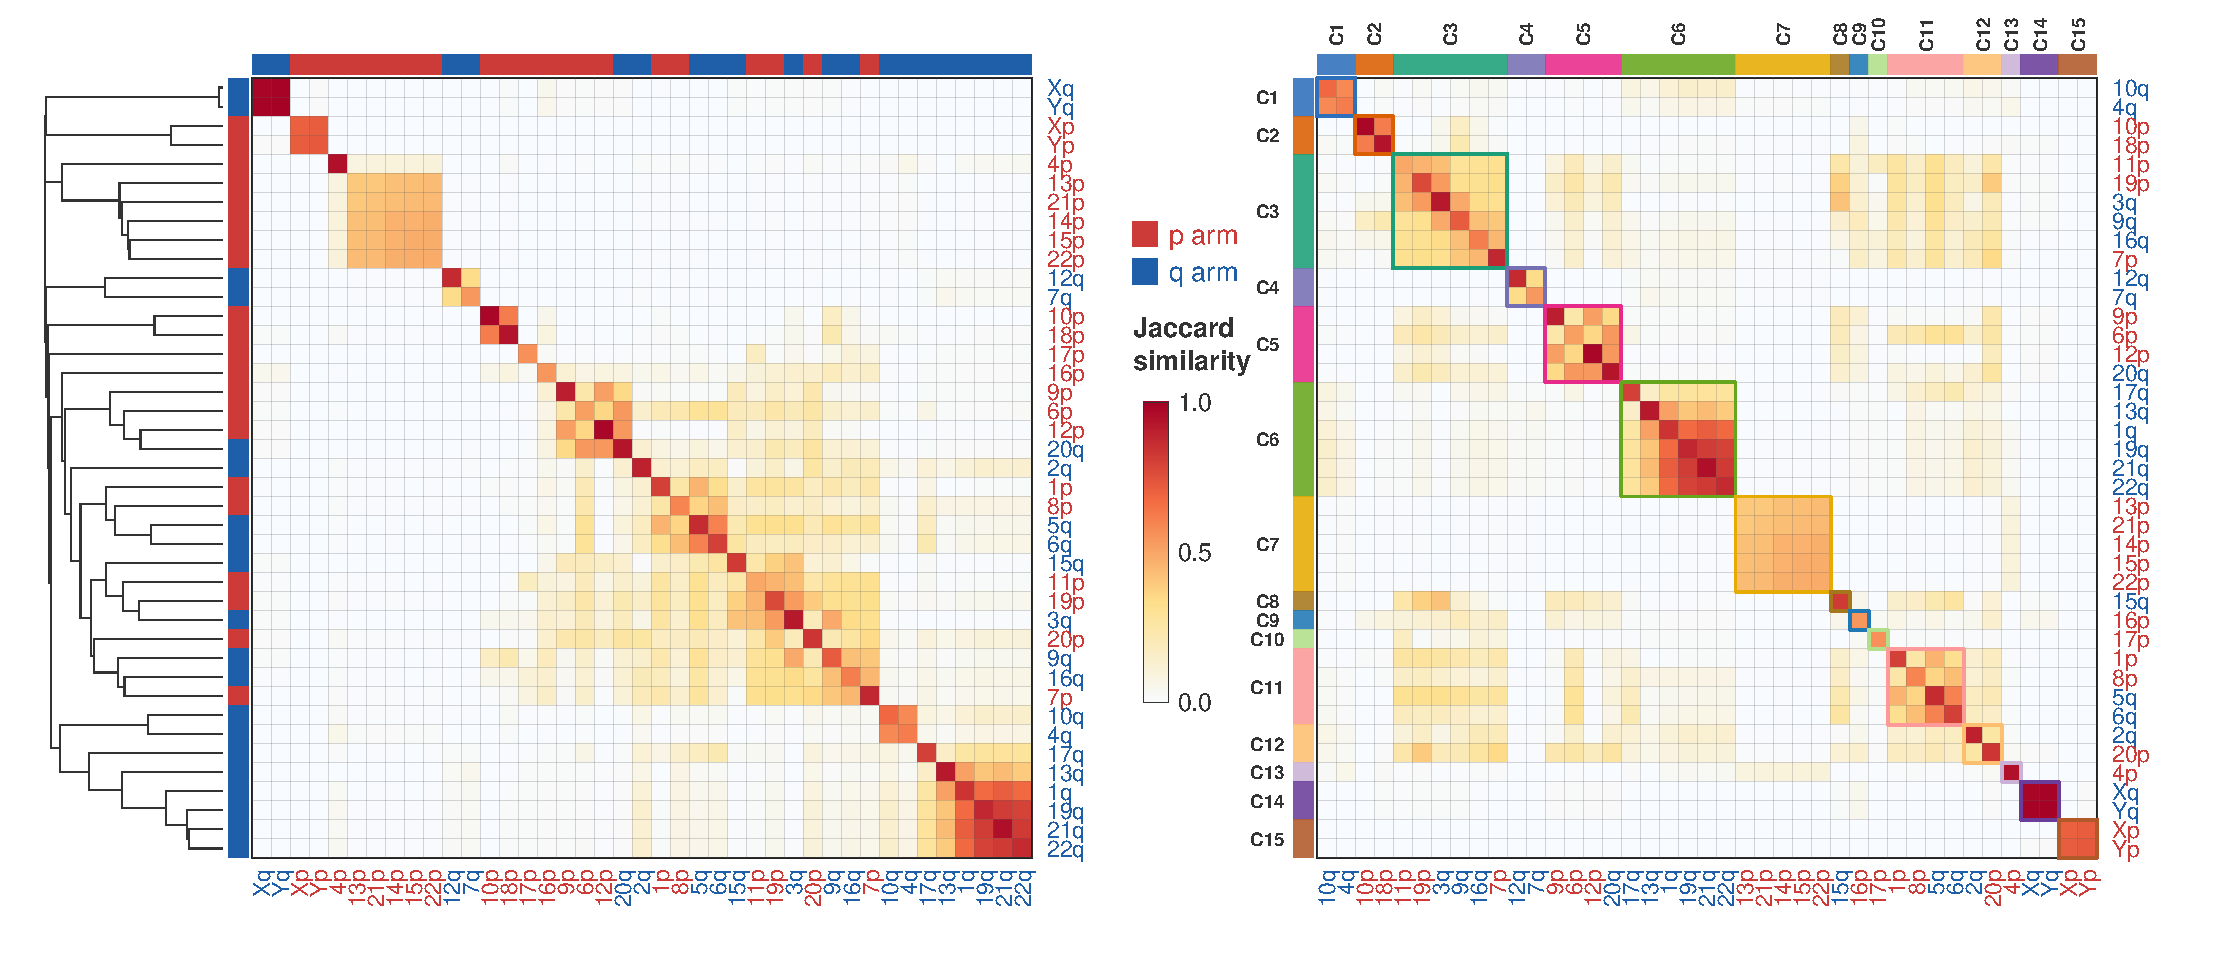
\includegraphics[width=\linewidth]{fig/MainFigures/Fig2bc_jaccard.pdf}
  \caption{\textbf{Pangenome similarity structure and communities.}
    \textbf{(A)} PGGB/odgi 2D layout of the all-subtelomere PHR graph (727,156
    layout nodes; main connected component). All 15,668 PHR flanks fall into a
    single component, so subtelomeres are linked across non-homologous
    chromosomes rather than partitioned by chromosome.
    \textbf{(B)} Arm-level Jaccard similarity heatmap ($41 \times 41$), shown
    twice. \emph{Left}, ordered by an average-linkage UPGMA dendrogram used as a
    display order for similar subtelomeric PHR profiles (p-arms red, q-arms
    blue), showing locally dense blocks on a broader similarity continuum.
    \emph{Right}, the same matrix ordered by the 15-community Leiden arm-level
    partition, with community colour bands. The blocks recover the known systems
    shown here: PAR1, PAR2, the acrocentric p-arms, 10p/18p and the 4q/10q DUX4
    pair, and show an enriched q-arm neighborhood exemplified by 22q, 21q, 19q,
    1q, 13q and 17q.}
  \label{fig:fig2}
\end{figure}

\begin{figure}[h!]
  \centering
  
\includegraphics[width=\linewidth]{fig/MainFigures/Fig3a_C1_chr4q.png}\\[1pt]
  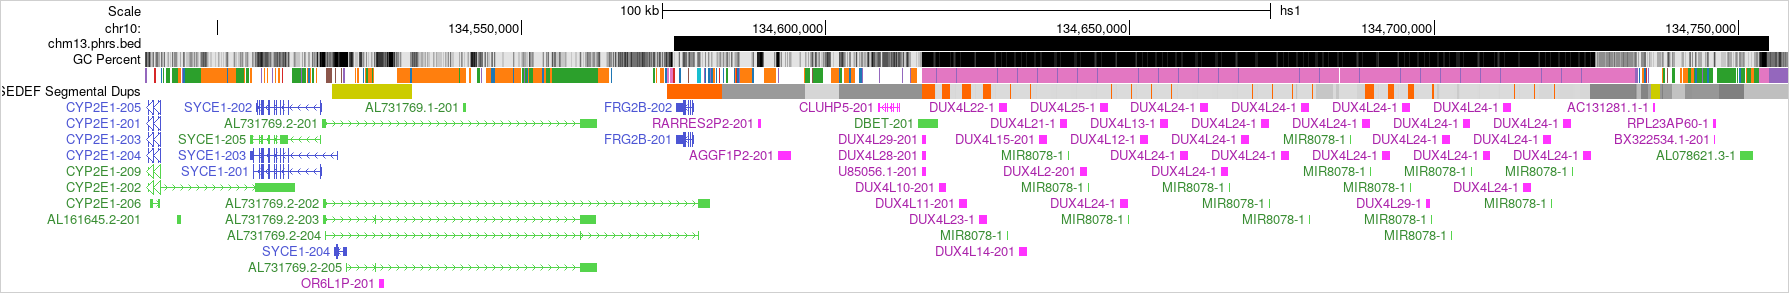
\includegraphics[width=\linewidth]{fig/MainFigures/Fig3a_C1_chr10q.png}\\[5pt]
  
\includegraphics[width=\linewidth]{fig/MainFigures/Fig3b_C2_chr10p.png}\\[1pt]
  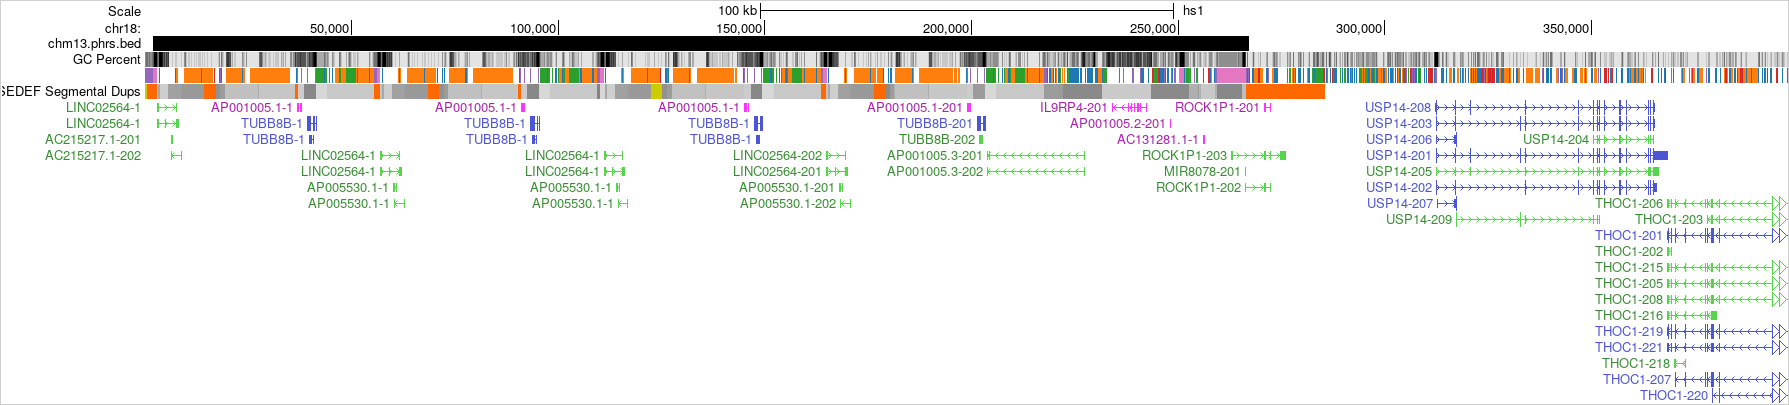
\includegraphics[width=\linewidth]{fig/MainFigures/Fig3b_C2_chr18p.png}\\[5pt]
  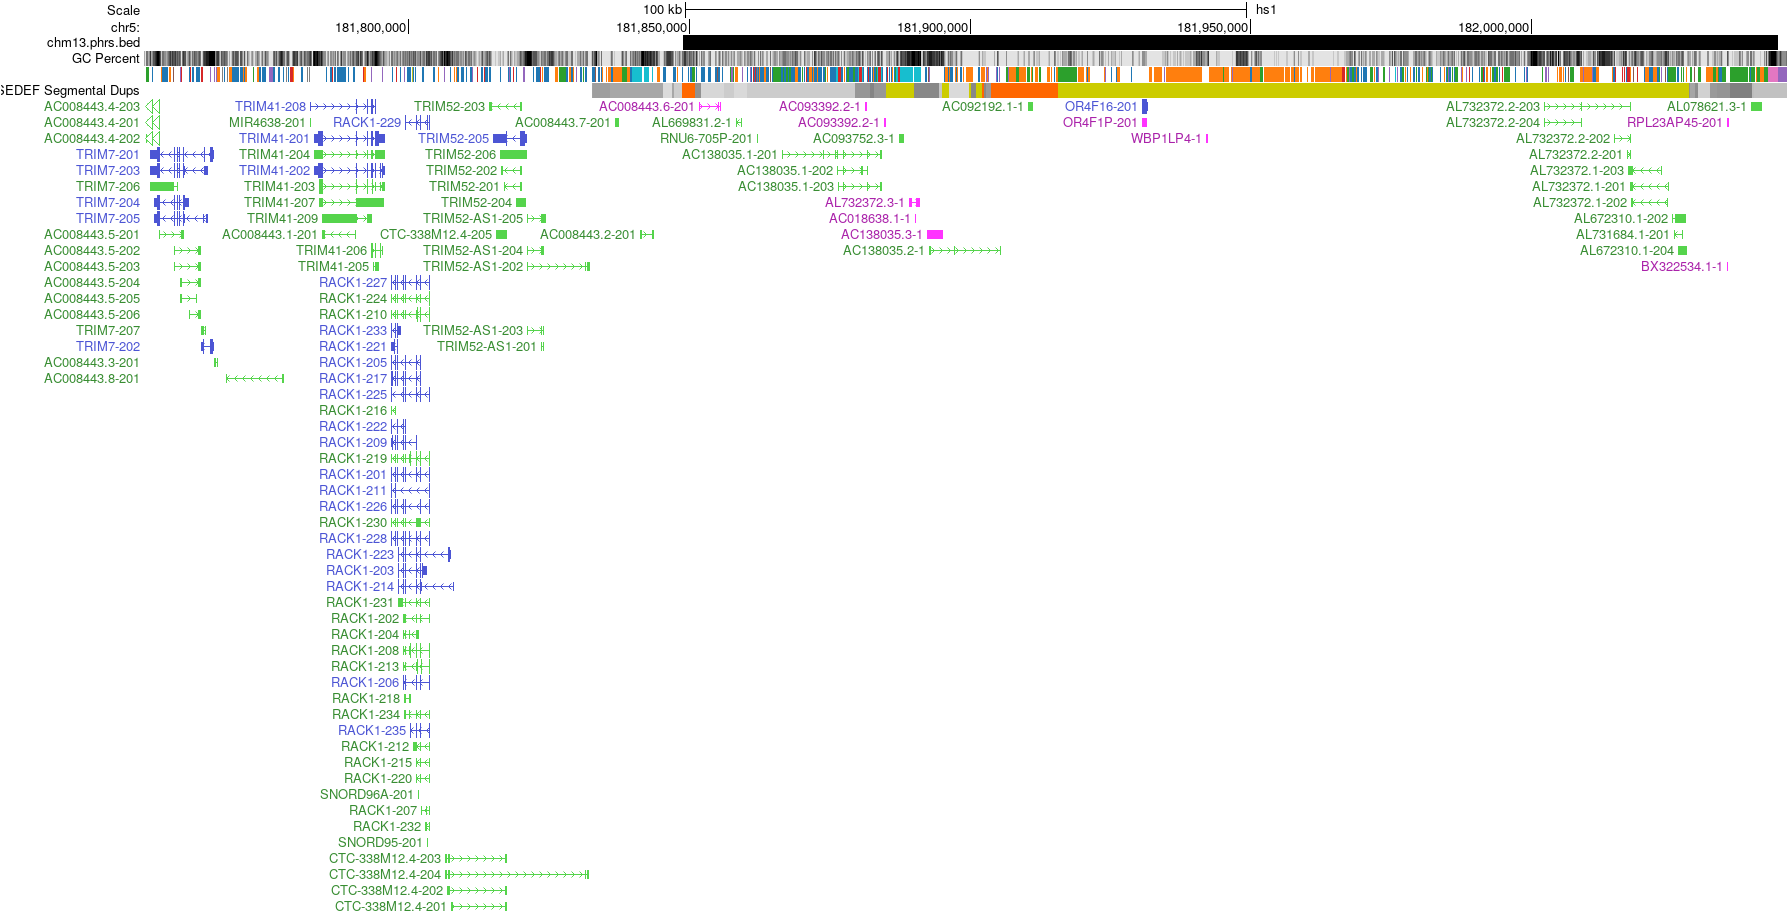
\includegraphics[width=\linewidth]{fig/MainFigures/Fig3c_C11_chr5q.png}\\[1pt]
  
\includegraphics[width=\linewidth]{fig/MainFigures/Fig3c_C11_chr6q.png}
  \caption{\textbf{Architecture of representative communities.}
    Sequence-level views (CHM13 coordinates, with PHR-BED, GC\%, segmental
    duplications and gene models) of three communities, so the duplicon content
    is legible without a genome browser.
    \textbf{(A)} Community C1 (4q/10q), the D4Z4/DUX4 system: homologous DUX4L
    macrosatellite arrays and FRG1/FRG2 paralog families on the 4q35 (top) and
    10q26 (bottom) ends, copy number 0--22 across haplotypes.
    \textbf{(B)} Community C2 (10p/18p), anchored by the TUBB8B tubulin gene
    array (tandem on 10p, top; single-copy on 18p, bottom).
    \textbf{(C)} Community C11 (5q/6q; 5q top, 6q bottom), built on the OR4F
    olfactory-receptor family and its pseudogenes.}
  \label{fig:fig3}
\end{figure}

\begin{figure}[h!]
  \centering
  % overpic 'percent' uses image WIDTH as 100 units for both axes, so the y of
  % the top edge = 100*(height/width): Fig4a~92.8, Fig4b~103.9, Fig4c(wide)~53.8.
  \begin{overpic}[width=0.50\linewidth]{fig/MainFigures/Fig4a_human_scatter.pdf}%
    \put(1,90){\textbf{\large\sffamily A}}\end{overpic}\hfill
  \begin{overpic}[width=0.447\linewidth]{fig/MainFigures/Fig4b_porec_community.pdf}%
    \put(1,100){\textbf{\large\sffamily B}}\end{overpic}\\[6pt]
  \begin{overpic}[width=\linewidth]{fig/MainFigures/Fig4c_mouse_zygotene.pdf}%
    \put(1,50){\textbf{\large\sffamily C}}\end{overpic}
  \caption{\textbf{Sequence similarity tracks three-dimensional proximity.}
    \textbf{(A)} Aggregate contact at PHR coordinates increases with sequence
    similarity in HG002 Pore-C. Each dot is one inter-chromosomal pair of
    pseudo-homolog regions (PHRs) within a single genome, so both axes derive
    from the same sample; \emph{x}, Jaccard sequence similarity of the two PHRs
    from the pangenome graph; \emph{y}, their length-normalised 3D contact at
    the PHRs' exact coordinates --- contact summed over the 50 kbp bin-pairs the
    two PHRs span, divided by that bin-pair count, so longer PHRs are not counted
    more (log scale, zero-contact pairs at the axis floor). Contact rises with
    similarity (descriptive pointwise Spearman
    $\rho = 0.381$, $n = 2{,}830$; line, linear fit).
    Replicates across a second genome and further assays are in Extended Data
    Fig.~\ref{fig:ed1}.
    \textbf{(B)} HG002 Pore-C contact matrix ordered by sequence community after
    observed/expected inter-chromosomal normalisation; within-community blocks
    dominate ($B/W = 0.056$). Matrix-level inference used row+column
    Mantel/permutation tests in Methods.
    \textbf{(C)} Mouse meiotic Hi-C (PHRs established de novo from B6 and CAST
    T2T assemblies, the whole pipeline re-run on a non-human mammal; 20 kbp,
    1 Mb flank). Left, one dot per inter-chromosomal mouse PHR sequence pair:
    zygotene contact (per-bin-pair length-normalised as in (A), log) rises with
    PHR Jaccard similarity. Right,
    mouse meiotic Hi-C supports a broad prophase-I sequence-to-contact
    association; the arm-pair-collapsed point estimate is largest at zygotene,
    but clustered zygotene-versus-flanking-stage contrasts do not establish a
    statistically resolved zygotene-specific peak.}
  \label{fig:fig4}
\end{figure}

\begin{figure}[h!]
  \centering
  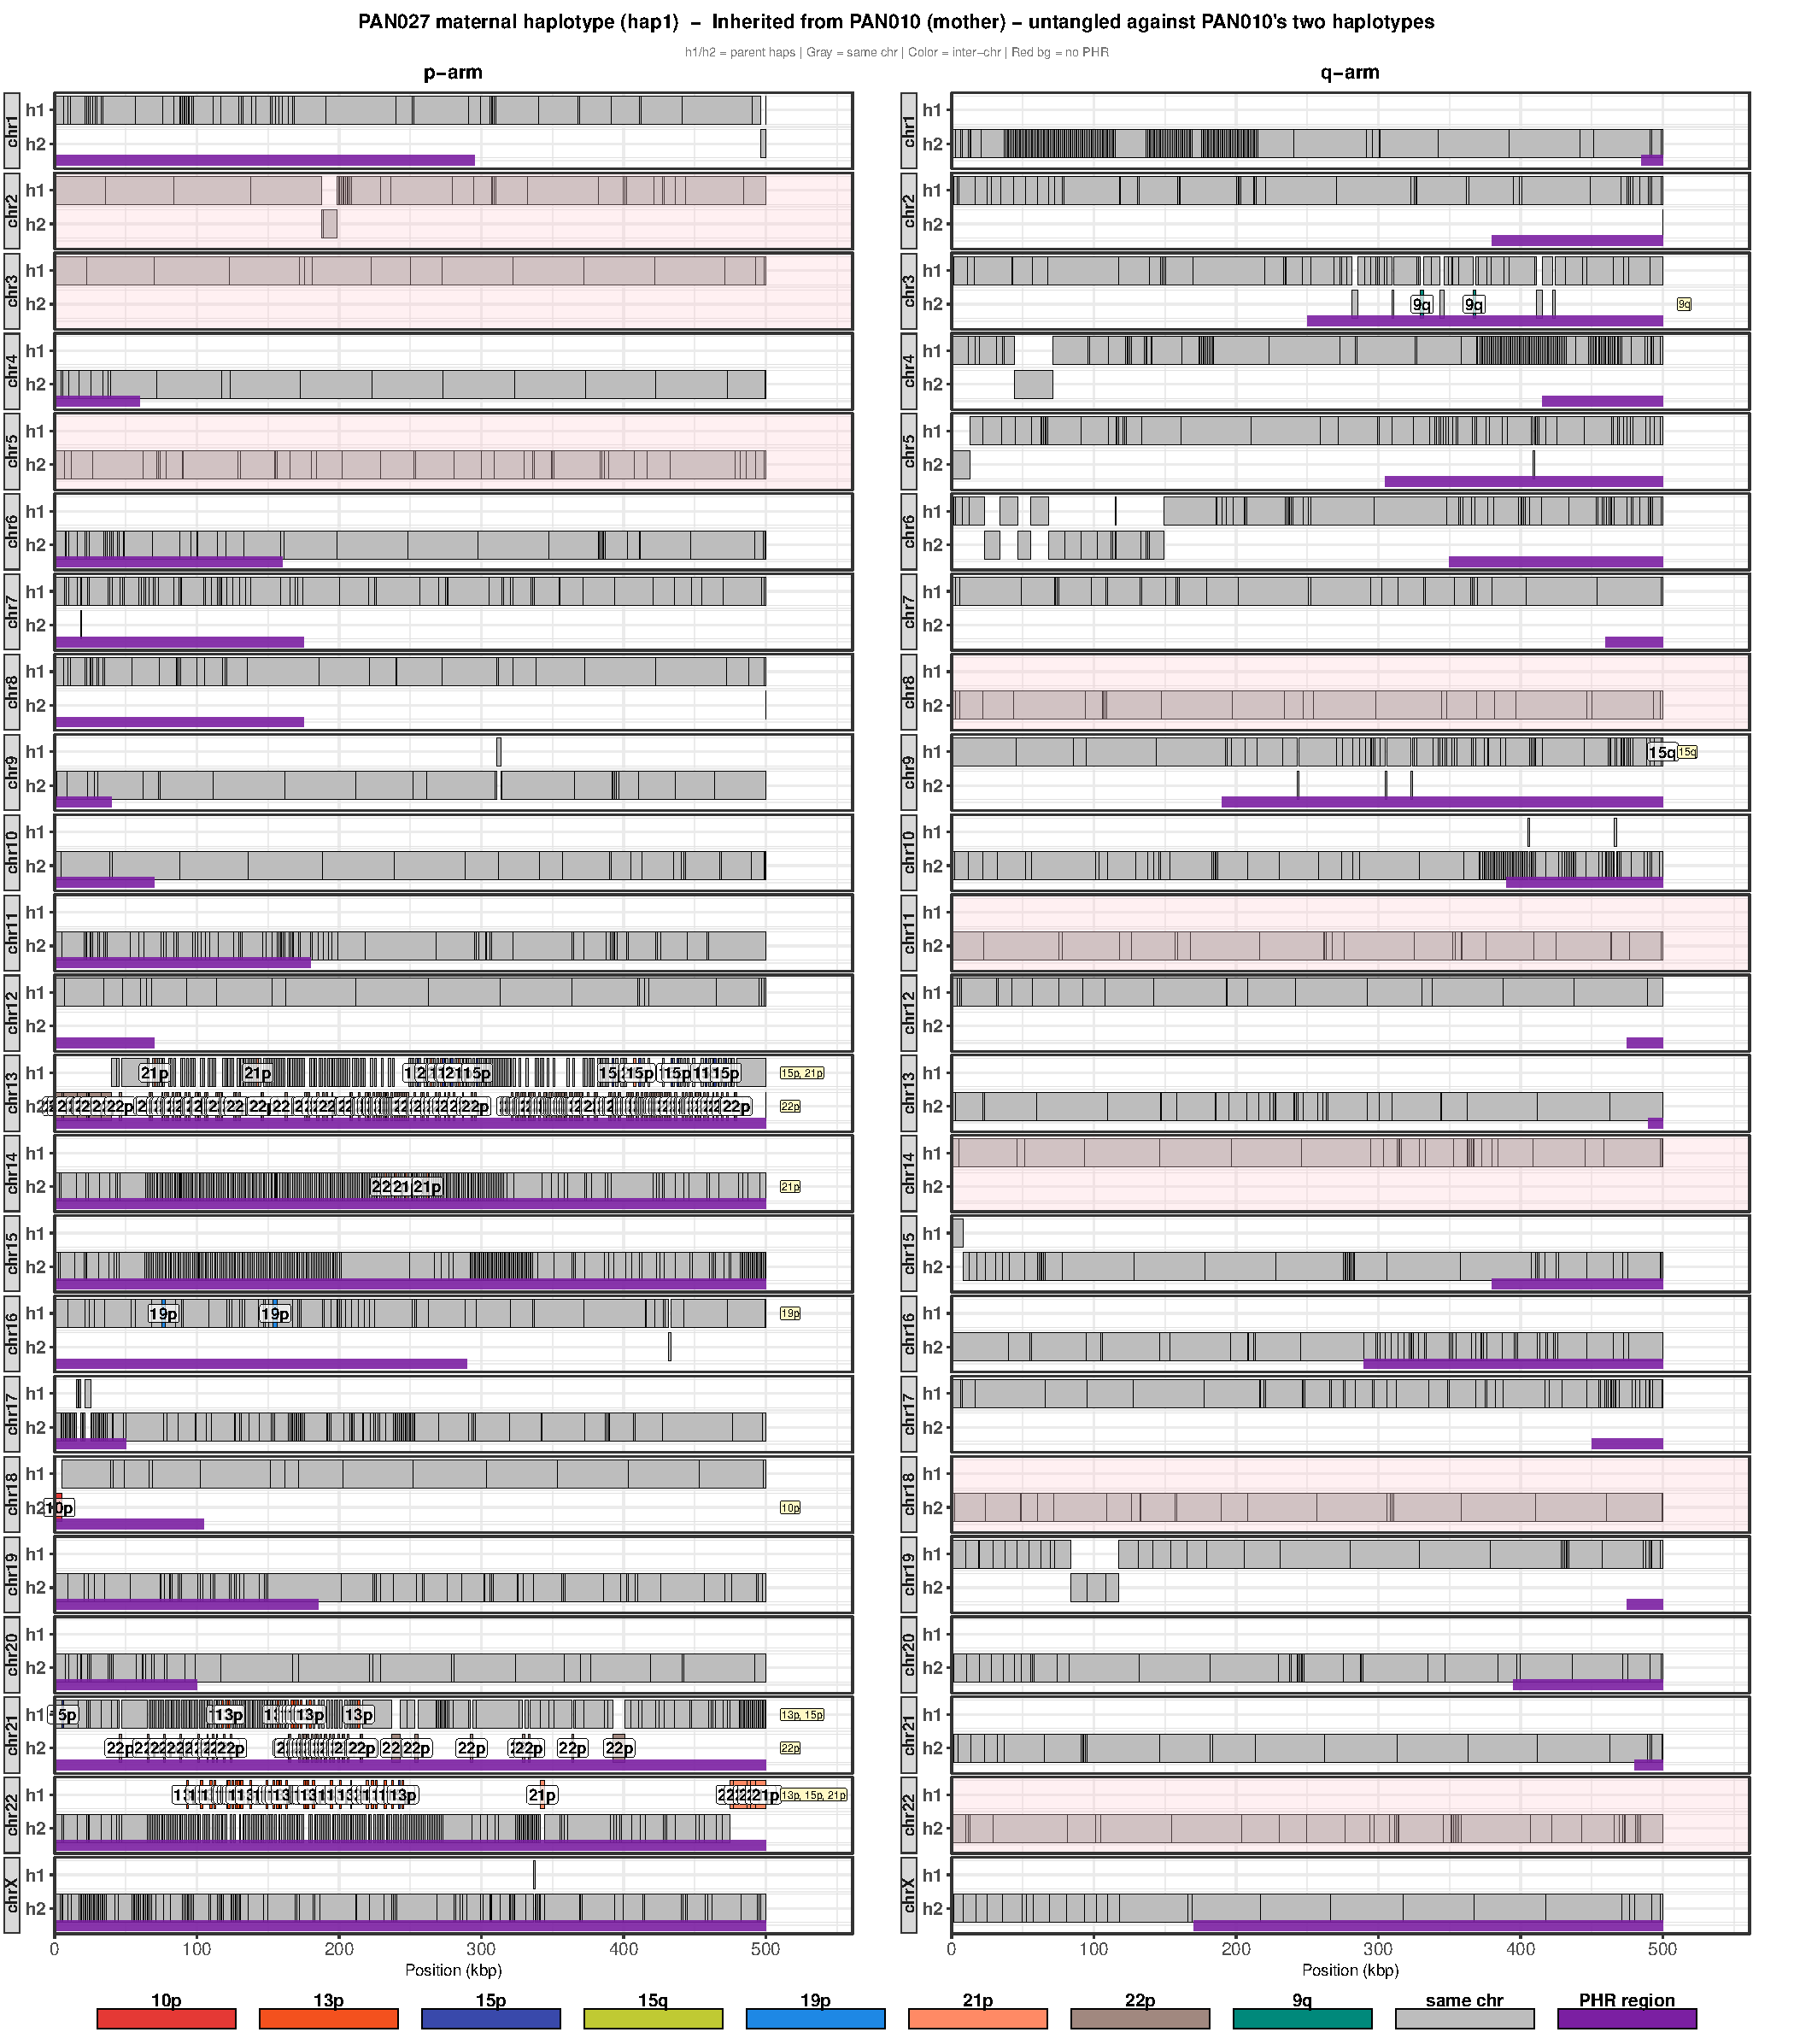
\includegraphics[width=\linewidth]{fig/MainFigures/Fig5_pedigree_untangle.pdf}
  \caption{\textbf{Pedigree-resolved candidate subtelomeric exchange.}
    Candidate inter-chromosomal subtelomeric patches in the WashU
    three-generation T2T pedigree. The PAN027 maternal haplotype (hap1,
    inherited from the mother PAN010) is untangled against PAN010's two
    haplotypes with \texttt{odgi untangle}, per chromosome arm (p-arms left,
    q-arms right; purple bars mark high-quality inter-chromosomal patch calls).
    Community labels were assigned after patch calling. Of 538 patch calls across
    three child-haplotype transmissions, 494 (92\%; Wilson 95\% CI 89.2--93.9\%)
    joined arms in the same independently inferred sequence-similarity community,
    above a marginal-aware Monte Carlo null (mean 77.0\%, 95\% CI 75.4--78.8\%;
    $p < 10^{-4}$), including crossover-like reciprocal exchanges and
    gene-conversion-like tracts. Cross-assembler validation (CEPH1463) is
    described in the main text.}
  \label{fig:fig5}
\end{figure}

\section*{Methods}
\label{secMethods}

\setcounter{figure}{0}

\subsection*{Sample selection and reference frame}

232 HPRC v2 individuals contributed haplotype-resolved assemblies, and
CHM13v2.0 was added as the closed-reference anchor.
The arm-flank census uses 465 assemblies: 464 HPRC haplotype assemblies
(232 individuals $\times$ 2) plus the haploid CHM13 assembly.
Superpopulation labels were assigned at the HPRC individual level
\cite{hprc_hprcv2_2025,Nurk2022,logsdon2025hgsvc}.

\subsection*{Sample exclusions}

Two exclusions are applied.
(i) GRCh38 contigs and CHM13\#0\#chrY (masked PAR1) are excluded from flank
extraction because they carry no telomeres compatible with the 500 kb anchored
extraction.
(ii) The chr18\_q flank from NA18982\#1 (JBKABS010000018.1, 84.4 Mb) is
excluded as a scaffolding chimera that fuses chr18 with 966 kb of chrX PAR1
across an NNN gap; confirmed by both wfmash and minimap2 v2.30 at MAPQ 60 and
by Flagger NNN/Hap labels.
No additional haplotype-level exclusions are applied.

\subsection*{Telomere-anchored 500 kb flank extraction}

For each haplotype assembly we extracted the terminal 500 kb of every contig
classified as p- or q-arm telomere-bearing (contig length $\geq 1$ Mb),
producing 18,827 flanks across 48 arms.
pq-classification at \texttt{pq-classification/contig\_classifications.tsv}.

\subsection*{wfmash all-vs-all alignment}

\texttt{wfmash v0.23.0-41-gb5f0ff1c -p 95 -t 48 --quiet}; each flank serves
as target in turn \cite{Guarracino2023}.
In a panmictic population most pairwise alignments are redundant; transitive
closure of the sampled fraction recovers effectively the same sequence graph as
exhaustive all-vs-all alignment.

\subsection*{Implicit pangenome graph and IMPG transitive closure}

The all-vs-all PAF set is the implicit pangenome graph; IMPG \texttt{query -x}
computes reachability
\cite{pangenome_graphs_impg_IMPG2023}.
Realised sampling rate 11.6\% (12\% rounded) sits $230\times$ above the
Erd\H{o}s and R\'{e}nyi connectivity threshold
$p^{*} = \log(n)/n = 5.2 \times 10^{-4}$ for $n = 18827$, justifying the
absence of chromosomal partitioning.

\subsection*{PHR detection}

IMPG sliding-window scan: identity $\geq 95\%$, $\geq 5$ alignments per
chromosome on $\geq 2$ different chromosomes, total aligned length per window
$\geq 3$ kb.
Output: 15,668 PHRs (83.2\% of flanks), 41 of 48 arms.

\subsection*{Pangenome graph and Jaccard similarity}

\texttt{pggb -p 95 -D /scratch}; \texttt{odgi similarity --all -P} over the
15,668 sequences yields the $15668 \times 15668$ Jaccard matrix
\cite{Garrison2024pggb,pangenome_graphs_impg_GuarracinoHeumos2022,andreace2023pangenome,heumos2024nfcore}.
The single connected component is rendered with \texttt{odgi layout} +
\texttt{odgi draw} (Fig.~\ref{fig:fig2}A).

\subsection*{Arm-level distance matrix}

Mean pairwise sequence-level Jaccard distance within each arm pair
(\texttt{hprcv2.1Mb.subtelo.arm\_dist\_matrix.tsv}).

\subsection*{Community detection (Leiden)}

Arm-level communities were inferred from the 41-arm Jaccard distance matrix
after converting distances to graph weights $w_{ij} = \exp(-d_{ij} /
\text{median}(d))$ and scanning Leiden resolution from 0.1 to 3.0.
The selected arm-level operating point was the maximum-silhouette 15-community
partition at resolution 1.16; the same community count was obtained across
resolutions 1.13--1.18.
Sequence-level communities were inferred from a k-nearest-neighbor graph on the
cached 15,668-sequence distance matrix.
The reported 50-community sequence partition uses the constrained operating
point $k_{\mathrm{NN}} = 75$, resolution 0.8; the unconstrained modularity
maximum in the scan gives a finer 148-community partition.
These scans evaluate resolution dependence on fixed similarity matrices and are
not a formal sample-resampling stability analysis.

\subsection*{UPGMA dendrogram}

For display and algorithmic comparison, we also ordered the arm-level matrix by
average-linkage hierarchical clustering using \texttt{hclust(..., method =
"average")}.
Cutting the same arm-level distance matrix into 14 UPGMA clusters gave mean
silhouette 0.342 and exact agreement with 12 of the 15 Leiden communities.
We use this dendrogram as a heatmap ordering and method comparison, not as a
phylogenetic model.

\subsection*{Neighbour-joining tree and character-level bootstrap}

We also audited an exploratory neighbour-joining and PHR-resampling analysis
used in earlier drafts.
That analysis resamples rows of a collapsed per-PHR cross-chromosome involvement
table, rebuilds an arm-level surrogate distance matrix, and recomputes NJ and
UPGMA trees.
It does not resample the full 15,668-sequence Jaccard matrix and is therefore
not used as evidence for the Leiden communities or for a hard q-arm partition.
Under this chromosome-granular surrogate, the illustrative six-arm
q-neighborhood has low support, so we treat the q-arm pattern as an enriched
neighborhood in the similarity matrix rather than as a bootstrap-supported
grouping.

\subsection*{Hi-C, Pore-C and CiFi pipeline}

mcool inputs at 5, 10, 20, 50 and 100 kb; per-haplotype mode preserves
maternal and paternal contigs as separate arms.
Hi-C, Pore-C, CiFi, Dip-C and sperm scHi-C were reprocessed with multi-mappers
retained because default MAPQ-filtered deposited maps remove the paralogous
subtelomeric signal-bearing sequence.
Under this policy, each multi-mapped molecule contributes one primary placement
rather than all possible placements.
PHR-internal contacts are therefore aggregate coordinate-level measurements and
not read-level truth sets.
The adjacent flanking unique-sequence analyses provide the principal control
against broad MAPQ0-driven inflation.
Pointwise Spearman correlations are reported as descriptive effect sizes
because PHR-pair observations share chromosome arms, PHRs, matrix rows/columns
and read-placement histories.
Matrix-level inference used row+column Mantel/permutation tests; finite
permutation floors are reported when no permutation exceeds the observed
statistic.
Observed/expected inter-chromosomal normalisation was used for community-ordered
contact matrices \cite{hic3d_dixon2012,hic3d_imakaev2012,Ulahannan2019,hic3d_cifi2025}.
The pointwise Spearman correlations take each inter-chromosomal PHR sequence
pair as a point, correlating its pangenome-graph Jaccard with its
length-normalised Hi-C/Pore-C contact at the pair's exact coordinates within one
genome: HG002 Pore-C in Fig.~\ref{fig:fig4}A ($\rho = 0.381$, $n = 2{,}830$) and,
as replicates in Extended Data Fig.~\ref{fig:ed1}, CHM13 Hi-C ($\rho = 0.716$,
$n = 652$), HG002 Hi-C ($\rho = 0.662$, $n = 2{,}544$) and HG002 CiFi
($\rho = 0.191$, $n = 2{,}757$; the sparsest assay, hence the weakest signal);
all at 50 kbp via \texttt{sequence\_hic\_correlation.py}.
The community-ordered Pore-C matrix of Fig.~\ref{fig:fig4}B ($B/W = 0.056$) is
at 50 kb.

\subsection*{Reproducibility from deposited data}

Standard deposited Hi-C MCool/Juicer files (default MAPQ $\geq 30$) do not
preserve the inter-arm signal because the high-identity PHR sequence is masked
at the deposited mapping stage.
We re-aligned all Hi-C, Pore-C, CiFi and Dip-C data from raw FASTQ against the
corresponding T2T reference (CHM13v2.0 or matched HPRC v2 haplotype) with
multi-mappers retained.
The re-alignment workflows and command lines are included in the public
analysis-code repository.
Deposited processed files generated with default MAPQ filters do not preserve
the inter-arm signal.

\subsection*{Exclusion controls (multi-resolution Mantel walk)}

Five exclusion sets (no acrocentric p-arms, no sex chromosomes, no acrocentric
p plus sex, no all-acrocentric plus sex, no strongest community) applied at all
five mcool resolutions.
The resulting Mantel $\rho$ trajectory rises with confound removal: HG002
$0.66 \to 0.80$, HG02148 $0.15 \to 0.72$, CHM13 $0.66 \to 0.85$, NA19036
$0.27 \to 0.79$
\cite{hic3d_alavattam2019,hic3d_wolff2018,hic3d_deshpande2022}.

\subsection*{Single-cell 3D}

Dip-C in 16 GM12878 cells \cite{Tan2018} (17 raw cells; cell 12 excluded as
a duplicate of cell 10 by shared SRR7226706 long-insert library) remapped to
T2T-CHM13v2.0; sperm scHi-C in 20 cells
\cite{Xu2025,hic3d_scnanoHiC2023,hic3d_scnanoHiC2_2025,hic3d_kitamura2025}.
PBMC Dip-C negative control: 18 cells from the public Dip-C dataset
\cite{Tan2018}, with PHR coordinates projected from CHM13 to hg19 via impg,
yielding $W/B = 0.983$ and $p = 0.305$.
$S_{\mathrm{all}}$ negative control: pooled 7 zero-signal arms.

\subsection*{Mouse pipeline}

Repetition of the project on a non-human mammal.
B6 and CAST T2T assemblies \cite{Francis2025}; telomere-anchored flanks;
1/2/4 Mb window sweep (30/49 mouse PHRs saturate the 1 Mb window);
2-community arm-level partition; per-PHR-pair Spearman of length-normalised
contact vs PHR Jaccard similarity at 20 kb (1 Mb flank), one value per meiotic
prophase stage.
Subtelomeric sequence similarity was positively correlated with
inter-chromosomal contact across leptotene, zygotene, pachytene and diplotene.
At 1 Mb and 50 kb resolution, exact PHR-pair correlations were similar across
stages (Spearman $\rho = 0.37$--0.43), while arm-pair-collapsed correlations
were higher ($\rho = 0.57$--0.71) with the largest point estimate at zygotene.
Direct clustered contrasts did not resolve a zygotene-specific peak, so we
treat the mouse data as evidence for a broad prophase-I sequence-to-contact
association rather than a stage-specific maximum.
\texttt{vegan::mantel} cross-check within $\pm 0.02$ \cite{Zuo2021}; the Python
and R implementations are included in the public analysis-code repository.

\subsection*{Pedigree odgi-untangle}

Pedigree patches were called from \texttt{odgi untangle nth-best=1} output by
merging contiguous child-flank intervals assigned to the same transmitting
parent chromosome and haplotype.
The high-quality WashU denominator comprised all inter-chromosomal patches with
\texttt{min\_score} $\geq 0.8$ and
$500\ \mathrm{bp} \leq \mathrm{size} \leq 100\ \mathrm{kb}$.
Leiden labels from the independently inferred HPRCv2 arm-level community graph
were assigned only after patch calling.
The primary statistic was the fraction of high-quality WashU patches whose query
and donor arms shared a Leiden community, tested against a permutation null
preserving per-arm patch-count marginals.
Within-community status was used to select mechanistic examples and, for
CEPH1463, as part of a conservative cross-assembler validation criterion
\cite{Cechova2025,Porubsky2025}. The classification implementation is included
in the public analysis-code repository.
Patch tract lengths interpreted alongside long-read primate meiotic
recombination (NCO 22--95 bp, CO-associated 318--688 bp)
\cite{pedigree_Porsborg2025primaterecom,pedigree_Joseph2024PRDM9indep}.
The within-Leiden fraction was tested against a permutation null preserving
per-arm patch-count marginals ($B = 10000$; per-community BH correction);
Wilson 95\% CI on 494/538 is 89.2--93.9\%. The permutation implementation is
included in the public analysis-code repository.

\subsection*{Software versions}

wfmash 0.23.0-41-gb5f0ff1c; impg commit 5b96025; pggb and odgi bundled;
samtools, bedtools and bgzip via conda; hicexplorer 3.7.4; R packages
\texttt{ape}, \texttt{vegan} and \texttt{cluster}.

\subsection*{Data and code availability}

Analysis code, manuscript source, figure-generation scripts, and vendored
figure inputs are available at \url{https://github.com/ekg/phrs}. HPRC v2
assemblies, CHM13v2.0, WashU pedigree assemblies, CEPH1463 assemblies, and
published 3D-genome datasets are available from their cited public releases and
accessions; accession-level identifiers are listed with the corresponding
citations and source-data tables.
The public repository includes re-alignment workflows and command lines for
Hi-C, Pore-C, CiFi and Dip-C. These workflows start from the cited public
raw-read datasets; deposited processed files generated with default MAPQ
$\geq 30$ filters are insufficient to reproduce the inter-arm signal.

\subsection*{Limitations}

(i) Bulk Hi-C is somatic LCL, not germline meiotic; (ii) no genome-wide LAD or
Lamin B1 ChIP-seq in matched germline cell types; (iii) a PHR-level comparison
of Lalli 2025 T2T-CHM13 short-read cM/Mb estimates with our cross-arm affinity
metric shows an apparent anti-correlation only before filtering and collapses
after seven low-callability acrocentric/PAR arms are excluded; (iv) the 12\%
wfmash sampling rate is justified by Erd\H{o}s
and R\'{e}nyi connectivity but rests on the chosen 95\% identity threshold; (v)
flank size truncation at 500 kb may underestimate PHR length; (vi) Hi-C N is
small (six individuals) and confidence intervals are correspondingly wide.
Confidence intervals on all headline correlations are reported where supported
by the completed analyses, together with the Monte Carlo permutation null for
the pedigree within-community fraction (observed $p < 10^{-4}$).

\bibliography{bibliography}

\clearpage

\section{Extended Data Figure Legends}

\setcounter{figure}{0}
\renewcommand{\thefigure}{ED\arabic{figure}}

\begin{figure}[htb!]
  \centering
  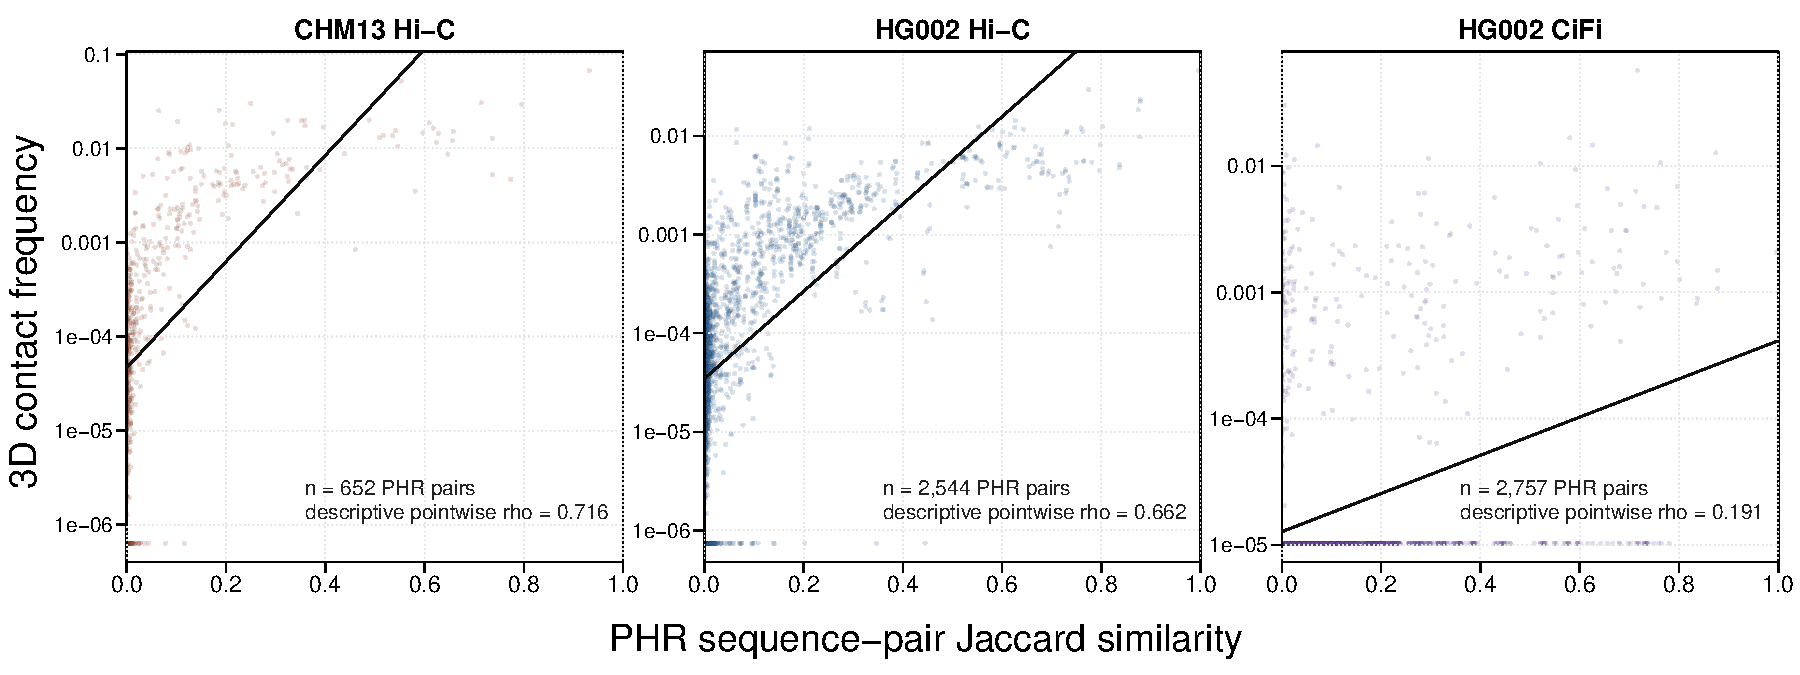
\includegraphics[width=\linewidth]{fig/ExtendedDataFigures/ED_Fig1_human_contacts.pdf}
  \caption{\textbf{The sequence-to-3D relationship replicates across genomes and
    contact assays.} Three companions to Fig.~\ref{fig:fig4}A, by the same
    all-points method (each dot is one inter-chromosomal PHR sequence pair within
    a single genome; \emph{x}, pangenome-graph Jaccard similarity; \emph{y}, mean
    3D contact per 50 kbp bin-pair the two PHRs span, as in Fig.~\ref{fig:fig4}A;
    log scale, zero-contact pairs at the axis floor; line, linear fit).
    Contact rises with similarity in every panel, reported as descriptive
    pointwise Spearman effect sizes:
    CHM13 Hi-C (a second genome; $\rho = 0.716$, $n = 652$), HG002 Hi-C (same
    genome as Fig.~\ref{fig:fig4}A, different assay; $\rho = 0.662$,
    $n = 2{,}544$), and HG002 CiFi ($\rho = 0.191$, $n = 2{,}757$; CiFi is the
    sparsest assay, $\sim$90\% of pairs zero-contact, hence the weakest
    directionally concordant signal).}
  \label{fig:ed1}
\end{figure}

\end{document}
